\documentclass{standalone}
\usepackage{tikz}
\usetikzlibrary{patterns, positioning}


\begin{document}
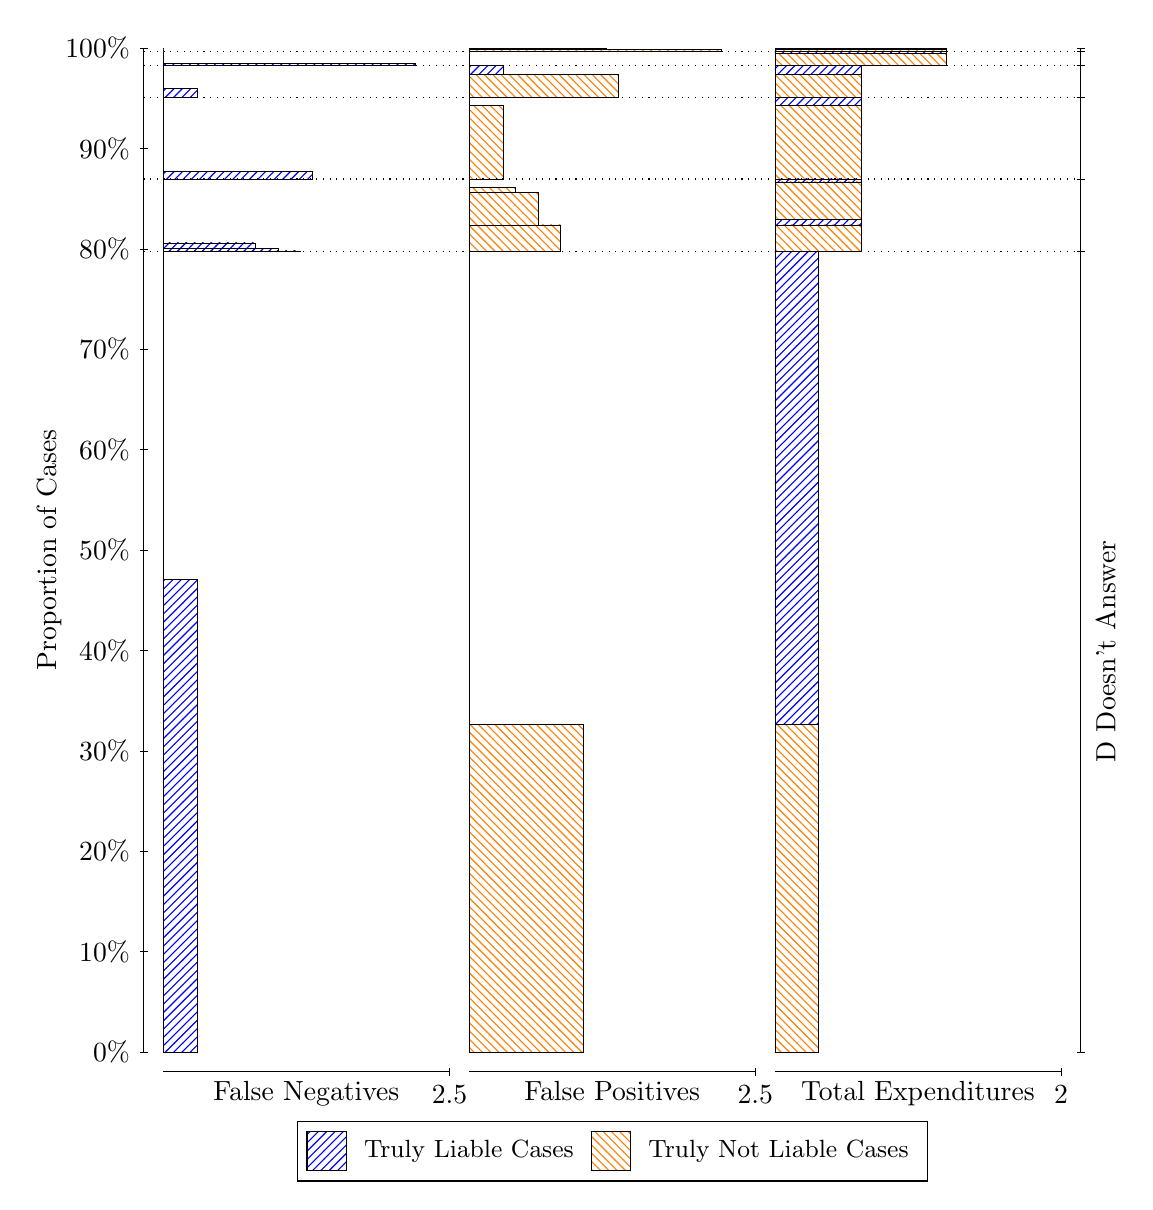
\begin{tikzpicture}
\draw[black, very thin] (1.5,1.75) -- (1.5,14.5);
\node[rotate=90, text=black, anchor=center] at (0.3, 8.125) {Proportion of Cases};
\draw[black, very thin] (1.45,1.75) -- (1.55,1.75);
\node[text=black, anchor=east] at (1.45, 1.75) {0\%};
\draw[black, very thin] (1.45,3.025) -- (1.55,3.025);
\node[text=black, anchor=east] at (1.45, 3.025) {10\%};
\draw[black, very thin] (1.45,4.3) -- (1.55,4.3);
\node[text=black, anchor=east] at (1.45, 4.3) {20\%};
\draw[black, very thin] (1.45,5.575) -- (1.55,5.575);
\node[text=black, anchor=east] at (1.45, 5.575) {30\%};
\draw[black, very thin] (1.45,6.85) -- (1.55,6.85);
\node[text=black, anchor=east] at (1.45, 6.85) {40\%};
\draw[black, very thin] (1.45,8.125) -- (1.55,8.125);
\node[text=black, anchor=east] at (1.45, 8.125) {50\%};
\draw[black, very thin] (1.45,9.4) -- (1.55,9.4);
\node[text=black, anchor=east] at (1.45, 9.4) {60\%};
\draw[black, very thin] (1.45,10.675) -- (1.55,10.675);
\node[text=black, anchor=east] at (1.45, 10.675) {70\%};
\draw[black, very thin] (1.45,11.95) -- (1.55,11.95);
\node[text=black, anchor=east] at (1.45, 11.95) {80\%};
\draw[black, very thin] (1.45,13.225) -- (1.55,13.225);
\node[text=black, anchor=east] at (1.45, 13.225) {90\%};
\draw[black, very thin] (1.45,14.5) -- (1.55,14.5);
\node[text=black, anchor=east] at (1.45, 14.5) {100\%};

\draw[black, very thin] (13.4,1.75) -- (13.4,14.5);
\draw[black, very thin] (13.35,1.75) -- (13.45,1.75);
\node[anchor=west] at (13.35, 1.75) {};
\draw[black, very thin] (13.35,11.92) -- (13.45,11.92);
\node[anchor=west] at (13.35, 11.92) {};
\draw[black, very thin] (13.35,12.837) -- (13.45,12.837);
\node[anchor=west] at (13.35, 12.837) {};
\draw[black, very thin] (13.35,13.87) -- (13.45,13.87);
\node[anchor=west] at (13.35, 13.87) {};
\draw[black, very thin] (13.35,14.279) -- (13.45,14.279);
\node[anchor=west] at (13.35, 14.279) {};
\draw[black, very thin] (13.35,14.455) -- (13.45,14.455);
\node[anchor=west] at (13.35, 14.455) {};
\draw[black, very thin] (13.35,14.5) -- (13.45,14.5);
\node[anchor=west] at (13.35, 14.5) {};

\draw[black, very thin, pattern color=blue, pattern=north east lines] (1.75,1.75) rectangle (2.186,7.7565);
\draw[black, very thin, pattern color=orange, pattern=north west lines] (1.75,7.7565) rectangle (1.75,11.92);
\draw[black, very thin, pattern color=blue, pattern=north east lines] (1.75,11.92) rectangle (3.494,11.925);
\draw[black, very thin, pattern color=blue, pattern=north east lines] (1.75,11.925) rectangle (3.2033,11.958);
\draw[black, very thin, pattern color=blue, pattern=north east lines] (1.75,11.958) rectangle (2.9127,12.025);
\draw[black, very thin, pattern color=orange, pattern=north west lines] (1.75,12.025) rectangle (1.75,12.837);
\draw[black, very thin, pattern color=blue, pattern=north east lines] (1.75,12.837) rectangle (3.6393,12.938);
\draw[black, very thin, pattern color=orange, pattern=north west lines] (1.75,12.938) rectangle (1.75,13.87);
\draw[black, very thin, pattern color=blue, pattern=north east lines] (1.75,13.87) rectangle (2.186,13.987);
\draw[black, very thin, pattern color=orange, pattern=north west lines] (1.75,13.987) rectangle (1.75,14.279);
\draw[black, very thin, pattern color=blue, pattern=north east lines] (1.75,14.279) rectangle (4.9473,14.306);
\draw[black, very thin, pattern color=orange, pattern=north west lines] (1.75,14.306) rectangle (1.75,14.455);
\draw[black, very thin, pattern color=orange, pattern=north west lines] (1.75,14.455) rectangle (1.75,14.481);
\draw[black, very thin, pattern color=blue, pattern=north east lines] (1.75,14.481) rectangle (1.75,14.5);
\draw[black, very thin, pattern color=orange, pattern=north west lines] (5.6333,1.75) rectangle (7.0867,5.9135);
\draw[black, very thin, pattern color=blue, pattern=north east lines] (5.6333,5.9135) rectangle (5.6333,11.92);
\draw[black, very thin, pattern color=orange, pattern=north west lines] (5.6333,11.92) rectangle (6.796,12.253);
\draw[black, very thin, pattern color=orange, pattern=north west lines] (5.6333,12.253) rectangle (6.5053,12.662);
\draw[black, very thin, pattern color=orange, pattern=north west lines] (5.6333,12.662) rectangle (6.2147,12.732);
\draw[black, very thin, pattern color=blue, pattern=north east lines] (5.6333,12.732) rectangle (5.6333,12.837);
\draw[black, very thin, pattern color=orange, pattern=north west lines] (5.6333,12.837) rectangle (6.0693,13.769);
\draw[black, very thin, pattern color=blue, pattern=north east lines] (5.6333,13.769) rectangle (5.6333,13.87);
\draw[black, very thin, pattern color=orange, pattern=north west lines] (5.6333,13.87) rectangle (7.5227,14.161);
\draw[black, very thin, pattern color=blue, pattern=north east lines] (5.6333,14.161) rectangle (6.0693,14.279);
\draw[black, very thin, pattern color=orange, pattern=north west lines] (5.6333,14.279) rectangle (5.6333,14.428);
\draw[black, very thin, pattern color=blue, pattern=north east lines] (5.6333,14.428) rectangle (5.6333,14.455);
\draw[black, very thin, pattern color=orange, pattern=north west lines] (5.6333,14.455) rectangle (8.8307,14.481);
\draw[black, very thin, pattern color=blue, pattern=north east lines] (5.6333,14.481) rectangle (7.3773,14.5);
\draw[black, very thin, pattern color=orange, pattern=north west lines] (9.5167,1.75) rectangle (10.062,5.9135);
\draw[black, very thin, pattern color=blue, pattern=north east lines] (9.5167,5.9135) rectangle (10.062,11.92);
\draw[black, very thin, pattern color=orange, pattern=north west lines] (9.5167,11.92) rectangle (10.607,12.253);
\draw[black, very thin, pattern color=blue, pattern=north east lines] (9.5167,12.253) rectangle (10.607,12.32);
\draw[black, very thin, pattern color=orange, pattern=north west lines] (9.5167,12.32) rectangle (10.607,12.799);
\draw[black, very thin, pattern color=blue, pattern=north east lines] (9.5167,12.799) rectangle (10.607,12.837);
\draw[black, very thin, pattern color=orange, pattern=north west lines] (9.5167,12.837) rectangle (10.607,13.769);
\draw[black, very thin, pattern color=blue, pattern=north east lines] (9.5167,13.769) rectangle (10.607,13.87);
\draw[black, very thin, pattern color=orange, pattern=north west lines] (9.5167,13.87) rectangle (10.607,14.161);
\draw[black, very thin, pattern color=blue, pattern=north east lines] (9.5167,14.161) rectangle (10.607,14.279);
\draw[black, very thin, pattern color=orange, pattern=north west lines] (9.5167,14.279) rectangle (11.697,14.428);
\draw[black, very thin, pattern color=blue, pattern=north east lines] (9.5167,14.428) rectangle (11.697,14.455);
\draw[black, very thin, pattern color=orange, pattern=north west lines] (9.5167,14.455) rectangle (11.697,14.481);
\draw[black, very thin, pattern color=blue, pattern=north east lines] (9.5167,14.481) rectangle (11.697,14.5);
\draw[black, dotted] (1.5,11.92) -- (13.4,11.92);
\draw[black, dotted] (1.5,12.837) -- (13.4,12.837);
\draw[black, dotted] (1.5,13.87) -- (13.4,13.87);
\draw[black, dotted] (1.5,14.279) -- (13.4,14.279);
\draw[black, dotted] (1.5,14.455) -- (13.4,14.455);
\draw[black, very thin] (1.75,1.5) -- (5.3833,1.5);
\node[text=black, anchor=north] at (3.5667, 1.5) {False Negatives};
\draw[black, very thin] (5.3833,1.45) -- (5.3833,1.55);
\node[text=black, anchor=north] at (5.3833, 1.45) {2.5};

\draw[black, very thin] (5.6333,1.5) -- (9.2667,1.5);
\node[text=black, anchor=north] at (7.45, 1.5) {False Positives};
\draw[black, very thin] (9.2667,1.45) -- (9.2667,1.55);
\node[text=black, anchor=north] at (9.2667, 1.45) {2.5};

\draw[black, very thin] (9.5167,1.5) -- (13.15,1.5);
\node[text=black, anchor=north] at (11.333, 1.5) {Total Expenditures};
\draw[black, very thin] (13.15,1.45) -- (13.15,1.55);
\node[text=black, anchor=north] at (13.15, 1.45) {2};

\node[text=black, centered, rotate=90] at (13.72, 6.835) {D Doesn't Answer};






\draw (7.449999999999999,1.5) node[draw=none] (baseCoordinate) {};
\begin{scope}[align=center]
        \matrix[scale=0.5, draw=black, below=0.5cm of baseCoordinate, nodes={draw}, column sep=0.1cm]{
            \node[rectangle, draw, minimum width=0.5cm, minimum height=0.5cm, pattern color=blue, pattern=north east lines] {}; &
            \node[draw=none, font=\small, text=black] (B) {Truly Liable Cases}; &
            \node[rectangle, draw, minimum width=0.5cm, minimum height=0.5cm, pattern color=orange, pattern=north west lines] {}; &
            \node[draw=none, font=\small, text=black] (B) {Truly Not Liable Cases}; \\
            };
\end{scope}

\end{tikzpicture}
\end{document}